%==============================================================================
% Sjabloon poster bachproef
%==============================================================================
% Gebaseerd op document class `a0poster' door Gerlinde Kettl en Matthias Weiser
% Aangepast voor gebruik aan HOGENT door Jens Buysse en Bert Van Vreckem

\documentclass[a0,portrait]{hogent-poster}

% Info over de opleiding
\course{Bachelorproef}
\studyprogramme{toegepaste informatica}
\academicyear{2023-2024}
\institution{Hogeschool Gent, Valentin Vaerwyckweg 1, 9000 Gent}

% Info over de bachelorproef
\title{Onderzoek naar de compilatie en bind van een Coolgen programma via een Azure DevOps pipeline binnen de mainframe omgeving van ArcelorMittal Gent met proof of concept.}
\author{Dylan Vermeersch}
\email{dylan.vermeersch@student.hogent.be}
\supervisor{Dhr. Leendert Blondeel}
\cosupervisor{Dhr. Didier Marichal (ArcelorMittal Gent)}

% Indien ingevuld, wordt deze informatie toegevoegd aan het einde van de
% abstract. Zet in commentaar als je dit niet wilt.
\specialisation{Mainframe Expert}
\keywords{Coolgen, DevOps, pipeline, IBM DBB}
%\projectrepo{https://github.com/user/repo}

\begin{document}

\maketitle

\begin{abstract}
Dit onderzoek zal gaan over het uitwerken van een werkende Azure DevOps pipeline om Coolgen programma's te compileren en binden met behulp van IBM Dependency Based Build (DBB) en zijn ingebouwd framework. Er werd gezocht naar een oplossing om de mainframe omgeving van ArcelorMittal Gent te moderniseren om zo aantrekkelijker te zijn voor afgestudeerden en om gebruik te maken van de nieuwere technologieën binnen het mainframe landschap. In de proof of concept is er een proefopstelling opgezet zodat de Coolgen applicaties kunnen worden gecompileerd en gebind via een Azure pipeline. Op die manier hoeft de ontwikkelaar niet zelf de compilatie en/of bind te starten. Het verwachte resultaat is dat de pipeline een correcte compilatie en bind kan uitvoeren zonder dat de ontwikkelaar zelf iets moet uitvoeren op de mainframe omgeving en dat het versiebeheer volledig kan beheerd worden door Azure DevOps. Zo zal er een einde komen aan de vele stappen die nodig zijn om een compilatie en bind van een Coolgen programma uit te voeren ook zal er voortaan in een Git ondersteunende IDE gewerkt kunnen worden.
\end{abstract}

\begin{multicols}{2} % This is how many columns your poster will be broken into, a portrait poster is generally split into 2 columns

\section{Introductie}

Deze bachelorproef gaat over op welke manier er een Azure DevOps pipeline kan geïntegreerd worden binnen ArcelorMittal Gent om hun bestaande en toekomstige Coolgen programma's te compilen/binden. 
Dit onderzoek is begonnen omdat ArcelorMittal Gent graag hun mainframe omgeving wil moderniseren en automatiseren, meer bepaald gaat het in dit onderzoek over het automatiseren van de compile/bind van Coolgen programma's.

\section{Experimenten}

In dit onderzoek is er een proof of concept uitgevoerd, hierdoor zijn er een aantal experimenten uitgevoerd in functie daarvan. Zo is er geëxperimenteerd met de uiteindelijke Git workflow die gebruikt werd, er zijn experimenten met betrekking tot de compile en bind van een Cobol- en Coolgen programma. Als laatste zijn er experimenten uitgevoerd in verband met het afscheiden van Coolgen code en de gegenereerde Cobol code. Al deze experimenten waren een belangrijk onderdeel van het onderzoek en zijn tevens allemaal goed verlopen. 
\begin{itemize}
    \item Git workflow bepalen
    \item Coolgen/Cobol compile/bind realiseren
    \item Afscheiden Coolgen- en Cobol code
\end{itemize}
\begin{center}
    \captionsetup{type=figure}
    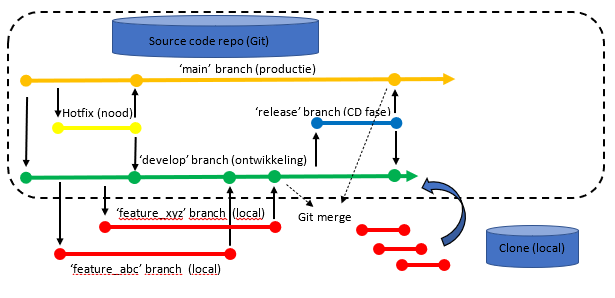
\includegraphics[width=1.0\linewidth]{Git_branching_strategy}
    \captionof{figure}{Git workflow bekomen door experimenten en onderzoek.}
    \label{fig:git workflow}
\end{center}


\section{Conclusies}

Alle experimenten zijn goed verlopen en de uiteindelijke resultaten zijn positief, hieruit kan er dus gehaald worden dat dit onderzoek aantoont dat het niet alleen mogelijk is om te werken met een DevOps pipeline binnen ArcelorMittal Gent maar dat het ook nog eens heel veel uitbreidingsmogelijkheden heeft. Uit de proof of concept is gebleken dat zo goed als alles binnen IBM Dependency Based Build aangepast kan worden aan de voorkeuren van ArcelorMittal Gent, zo is er zelfs een eigen meta data systeem binnen DBB gemaakt dat momenteel ook gebruikt wordt binnen ArcelorMittal Gent. 

\section{Toekomstig onderzoek}

Er is een goede basis gelegd voor toekomstig onderzoek naar een eventuele overgang van het huidige systeem naar een pipeline gebaseerd systeem, al dan niet met IBM DBB. Hoewel dit onderzoek al heel wat zaken aantoont te kunnen, is er nog bijkomend onderzoek nodig die bijvoorbeeld bepaald wat er nog aan functionaliteit ontbreekt binnen IBM DBB om eventueel deze zaken ook toe te voegen. Enkel als alle noodzakelijke functionaliteiten aanwezig zijn kan er effectief overgegaan worden naar een pipeline gebaseerd systeem voor het release management binnen ArcelorMittal Gent. 
\begin{center}
    \captionsetup{type=figure}
    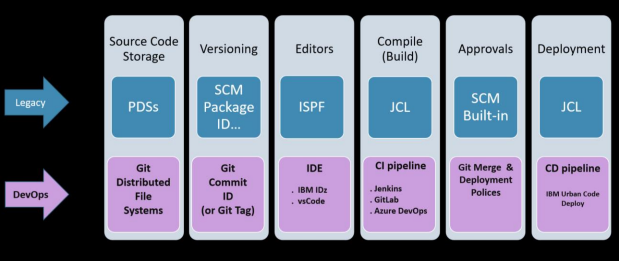
\includegraphics[width=1.0\linewidth]{Software_development_lifecycle}
    \captionof{figure}{Legacy (huidige) manier van werken binnen ArcelorMittal Gent en de DevOps (nieuwe) manier van werken.}
    \label{fig:oud vs nieuw}
\end{center}

\end{multicols}
\end{document}